\documentclass[oneside,final,14pt,a4paper]{extreport}

%# set the compiler XeLatex to use fontspec package
\usepackage{fontspec}
\usepackage{tempora}
\usepackage{hyperref}

\setmainfont{Times New Roman}

\usepackage{vmargin}
\setpapersize{A4}
\setmarginsrb{2.5cm}{2.2cm}{2.2cm}{2.2cm}{0pt}{10mm}{0pt}{13mm}
\usepackage{setspace}
\sloppy
\setstretch{1.5}
\usepackage{indentfirst}
\parindent=1.25cm

%%%%% ADDED TO SUPPORT TT BOLD FACES %%%%
\DeclareFontShape{OT1}{cmtt}{bx}{n}{<5><6><7><8><9><10><10.95><12><14.4><17.28><20.74><24.88>cmttb10}{}
\renewcommand{\ttdefault}{pcr}
%%%%% END %%%%%%%%%%%%%%%%%%%%%%%%%%%%%%% 
\usepackage{atbegshi,picture}
\usepackage[TT2,A1]{fontenc}
\usepackage[utf8]{inputenc}
\AtBeginShipout{\AtBeginShipoutUpperLeft{%
\put(\dimexpr\paperwidth-1cm\relax,-1.5cm){\makebox[0pt][r]{
\includegraphics[width=3cm]{figs/inno}}}%
}}


\usepackage[english]{babel}
\usepackage[style=ieee,autocite=inline]{biblatex}
\DefineBibliographyStrings{english}{bibliography = {References},}
\usepackage{blindtext}
\addbibresource{ref.bib}

\usepackage{xcolor}
\usepackage{pdfpages}
\newenvironment{bottompar}{\par\vspace*{\fill}}{\clearpage}
\usepackage{amsmath,amsfonts}
\usepackage{url}

\usepackage{amsthm}
\newtheorem{theorem}{Theorem}
\newtheorem{corollary}{Corollary}
\newtheorem{lemma}{Lemma}
\newtheorem{proposition}{Proposition}
\theoremstyle{definition}
\newtheorem{definition}{Definition}
\theoremstyle{remark}
\newtheorem*{remark}{Remark}
\theoremstyle{remark}
\newtheorem*{example}{Example}


\usepackage{titlesec}
\usepackage{float}
\usepackage{graphicx}
\graphicspath{{figs/}} %path to images
\usepackage{array}
\usepackage{multirow,array}
\usepackage{caption}
\usepackage{subcaption}
\usepackage{hyperref}
\usepackage{paralist}
\usepackage{listings}
\usepackage{zed-csp}
\usepackage{fancyhdr}
\usepackage{csquotes}
\usepackage{color}
% \usepackage{anyfontsize}
% \usepackage{mathptmx}
% \usepackage{t1enc}

\usepackage{chngcntr}
\usepackage{upgreek}
\usepackage{bm}
\usepackage{hyperref}
\usepackage{setspace}
\usepackage{booktabs}
\usepackage{multirow}
\usepackage{longtable}
\usepackage[font=singlespacing, labelfont=bf]{caption}
\counterwithout{table}{chapter}
\renewcommand{\thetable}{\Roman{table}}
%Hints
\newcommand\pic[1]{(Fig. \ref{\#1})} %Ref on figure
\newcommand\tab[1]{(Tab. \ref{\#1})} %Ref on table

\setlength{\headheight}{32.0976pt}
\usepackage{enumitem}
\newlist{inlinelist}{enumerate*}{1}
\setlist*[inlinelist,1]{%
label=(\arabic*),
}

\setcounter{secnumdepth}{4}
\captionsetup[table]{labelfont={normalfont}, name={TABLE}, labelsep={newline}}
\counterwithout{table}{chapter}
\renewcommand{\thetable}{\Roman{table}}
\setlength{\parindent}{2em}
\DeclareCaptionLabelSeparator{figSep}{.\quad}
\captionsetup[figure]{labelfont={normalfont}, name={Fig.}, labelsep=period}
\counterwithout{figure}{chapter}

\titleformat{\section}[hang]{\fontsize{20}{24}\selectfont\filcenter}{\Roman{section}}{1em}{}
\titleformat{\subsection}[hang]{\itshape}{\Alph{subsection}.}{1em}{}[]
\titleformat{\subsubsection}[runin]{\itshape}{\arabic{subsubsection})}{1em}{}[$:$]
\titlespacing{\subsubsection}{1em}{1em}{1em}
\titleformat{\paragraph}[runin]{\itshape}{\alph{paragraph})}{1em}{}[$:$\quad]
\titlespacing{\paragraph}{2em}{1em}{1em}

\pagestyle{fancyplain}

% remember section title
\renewcommand{\chaptermark}[1]%
{\markboth{\chaptername~\thechapter~--~\#1}{}}

% subsection number and title
\renewcommand{\sectionmark}[1]%
{\markright{\thesection\ #1}}

\rhead[\fancyplain{}{\bf\leftmark}]%
{\fancyplain{}{\bf\thepage}}
\lhead[\fancyplain{}{\bf\thepage}]%
{\fancyplain{}{\bf\rightmark}}
\cfoot{} %bfseries


\newcommand{\dedication}[1]



{\thispagestyle{empty}

\begin{flushleft}\raggedleft #1\end{flushleft}
}
\hypersetup{colorlinks=true, allcolors=black, citecolor=black}

\begin{document}

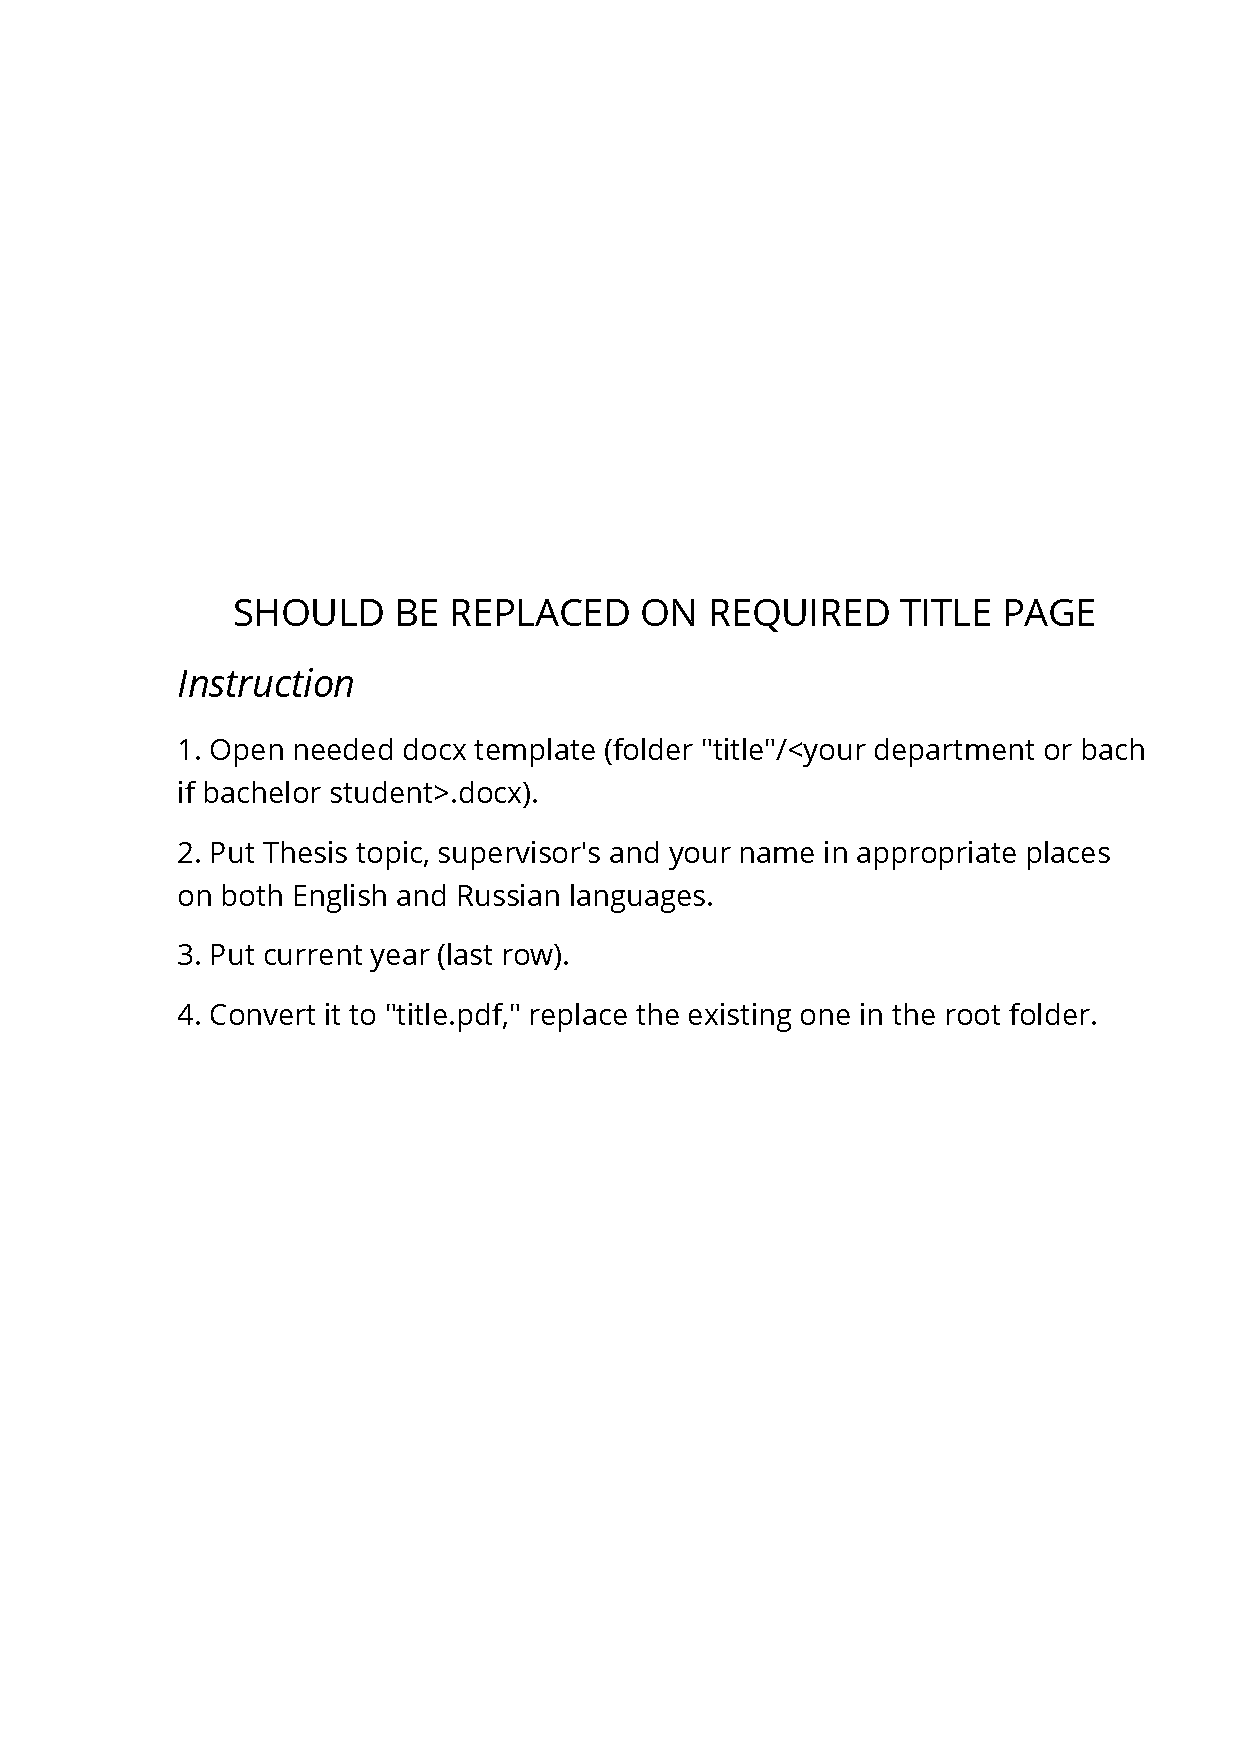
\includepdf[pages=-,offset=25.5mm -25.5mm]{title.pdf}
\tableofcontents
\listoftables
\listoffigures

\newpage
\setcounter{page}{8} % set manually an actual number from which introduction starts
\begin{abstract}

    BACKGROUND:
    The number of users of web services is increasing annually and, therefore, all developers aim to develop a high reliable software.
    However, no system can withstand any load, so site reliability engineers prepare for potential service failures by implementing various reliability practices to minimize associated risks.
    Feedback control system is a system that can give feedback about its current status so that engineers can react to it in advance the risks of a fall.

    OBJECTIVE:
    However, for feedback control systems developers face a problem that each reliability practice is configured in its own way and combinations of these settings can give different results in the reliability of the system.
    This paper outlines a web-service for reproducible load testing, visualization, and configuration of feedback control systems

    METHODS:
    The web-services was developed by using Kotlin and Spring Boot framework, and Kafka broker message was used for communication.
    Yandex tank was chosen as a high load generator for the ability to use several cores for load generation and a convenient API.
    Additionally, by using Angular framework I developed a UI interface for a more convenient and visual use of the service.

    RESULTS:
    The proposed service can handled services for configuration, executed load testing scenarios and provided real-time results as graphs.

    CONTRIBUTION AND APPLICABILITY:
    This service can be used in testing systems under various load scenarios with different configuration variants.
    These practices help to find the most effective combination of parameters that ensures optimal system performance.

\end{abstract}
\chapter{Introduction}
\label{chap:intro}
\chaptermark{Optional running chapter heading}
\section{Spacing \& Type}
\label{sec:section}

This is a section. This is a citation without brackets. and this is one with brackets \cite{A}. Multiple \cite{A,B,C} Here's a reference to a subsection: \ref{sec:subsection}. Citation of an online article \cite{D}. Citation of an online proceeding \cite{F}. The body of the text and abstract must be double-spaced except for footnotes or long quotations. Fonts such as Times Roman, Bookman, New Century Schoolbook, Garamond, Palatine, and Courier are acceptable and commonly found on most computers. The same type must be used throughout the body of the text. The font size must be 10 point or larger and footnotes\footnote{This is a footnote.} must be two sizes smaller than the text\footnote{This is another footnote.} but no smaller than eight points. Chapter, section, or other headings should be of a consistent font and size throughout the ETD, as should labels for illustrations, charts, and figures.

\subsection{Creating a Subsection}
\label{sec:subsection}

\subsubsection{Creating a Subsubsection}
\subsubsection{Creating a Subsubsection}
\subsubsection{Creating a Subsubsection}

\paragraph{This is a heading level below subsubsection}

And this is a quote: 
%
\begin{quote}
\blindtext
\end{quote}

\begin{figure}[hbt]
\centering

\includegraphics[]{figs/inno.png}
\caption{One kernel at $x_s$ (\emph{dotted kernel}) or two kernels at
$x_i$ and $x_j$ (\textit{left and right}) lead to the same summed estimate
at $x_s$. This shows a figure consisting of different types of
lines. Elements of the figure described in the caption should be set in
italics, in parentheses, as shown in this sample caption.}
\label{fig:example}
\end{figure}

This is a table:
% currsize is not set in the long table environment, so we need to set it before we set it up.
\makeatletter
\let\@currsize\normalsize
\makeatother

% tabular environments are set to be single-spaced in the  thesis class,  but long tables do not use tabular
% to get around this, set the spacing to single spacing at the start of the long table environment, and set it back to double-spacing at the end of it

\begin{longtable}{c|c|c}
\caption[This is the title I want to appear in the List of Tables]{This Is a Table Example} \label{tab:pfams} \\
\hline
A & B & C \\
\hline
\endfirsthead
\multicolumn{3}{@{}l}{} \\
\hline
A & B & C\\
\hline
\endhead
a1 & b1 & c1 \\
a2 & b2 & c2\\
a3 & b3 & c3\\
a4 & b4 & c4\\
\hline
\end{longtable}

The package ``upgreek'' allows us to use non-italicized lower-case greek letters. See for yourself: $\upbeta$, $\bm\upbeta$, $\beta$, $\bm\beta$. Next is a numbered equation:
\begin{align}
\label{eq:name}
\|\bm{X}\|_{2,1}={\underbrace{\sum_{j=1}^nf_j(\bm{X})}_{\text{convex}}}=\sum_{j=1}^n\|\bm{X}_{.,j}\|_2
\end{align}
The reference to equation (\ref{eq:name}) is clickable. 
\section[Theorems, Corollaries, Lemmas, Proofs, Remarks, Definitions and Examples]{Theorems, Corollaries, Lemmas, Proofs, Remarks, Definitions,and Examples}

\begin{theorem}
\label{thm:onlytheorem}
\blindtext
\end{theorem}

\begin{proof}
I'm a (very short) proof.
\end{proof}

\begin{lemma}
I'm a lemma.
\end{lemma}

\begin{corollary}
I include a reference to Thm. \ref{thm:onlytheorem}.
\end{corollary}

\begin{proposition}
I'm a proposition.
\end{proposition}

\begin{remark}
I'm a remark. 
\end{remark}

\begin{definition}
I'm a definition. I'm a definition. I'm a definition. I'm a definition. I'm a definition. I'm a definition. I'm a definition. I'm a definition. I'm a definition. I'm a definition. I'm a definition. 
\end{definition}

\begin{example}
I'm an example.
\end{example}


\section[Optional table of contents heading]{Section with\\ linebreaks in\\the
name}


\Blindtext[2]





\chapter{Literature Review}
\label{ch:lr}
\chaptermark{Second Chapter Heading}

This chapter investigates the reliability patterns and load testing.
It is organized in such way:
\begin{itemize}
    \item~\ref{sec:reliability} gives a brief overview of reliability patterns and their configurations.
    \item~\ref{sec:load_generation} provides the ideas about load testing and the comparison of modern load generation tools.
    \item~\ref{sec:review_conclusion} provides a conclusion of this chapter.
\end{itemize}


\section{Reliability patterns}\label{sec:reliability}
Reliability patterns ensure the stability and resiliency of high-performance systems.
Beyer B. et al.~\cite{google_sre}, examined a number of such strategies, including rate limiting, retry strategy, circuit breaker, and load balancing. Similar concepts are presented in ~\cite{reliability_patterns}, regarding circuit-breaker and retry patterns.
N. C. Mendonca, C. M. Aderaldo, J. Camara and D. Garlan~\cite{circuit_breaker} outlines that circuit-breaker can have several tuning parameters, such as the sleep window, the error percentage threshold, and others. But in real implementations, the set of tuning params may vary. This set may depend on the specific implementation or features of the programming language.

\begin{longtable}[c]{|p{4.5cm}|p{5.2cm}|p{5.3cm}|}
    \caption{Circuit breaker parameters for different implementations}
    \label{tab:patterns_table} \\
    \hline
    \textbf{Abstract parameter} & \textbf{Java (Resilience4j)} & \textbf{Python (Circuit breaker library)} \\
    \endhead
    \hline
    Timeout                     & maxWaitDuration       & recovery\_timeout                \\
    \hline
    Error Percent Threshold     & failureRateThreshold  & failure\_threshold               \\
    \hline
    Request Volume threshold    & minimumNumberOfCalls  & -                                \\
    \hline
    Sleep window                & slidingWindowSize     & -                                \\
    \hline
    - & \begin{tabular}[c]{@{}l@{}}
            recordExceptions,\\ slidingWindowType
    \end{tabular} & \begin{tabular}[c]{@{}l@{}}
                        expected\_exception,\\ fallback\_function
    \end{tabular} \\
    \hline
\end{longtable}

Table~\ref{tab:patterns_table} shows accordance of configuration parameters for abstract circuit breaker~\cite{circuit_breaker} and for real implementation in Java~\cite{resilience4j} and Python~\cite{circuitbreaker}. It shows that in real implementation we can have incomplete or more enhanced set of parameters and it's hard to create generic number of configuring params for all implementations.


\section{Load testing}\label{sec:load_generation}
To properly select a load generation tool, it is necessary to understand the goals of load testing. Daniel A.Menasc`e~\cite{load_testing_base} explains that load testing allows to measure the performance of a system: the average response time and throughput as a certain number of concurrent requests. Therefore, it is crucial for a load testing tool to generate a specified number of requests per second (RPS) and presents the results as the response time and the maximum RPS that the server can handle.
R. Abbas, Z. Sultan, and S. N. Bhatti~\cite{load_testing_tools} provide a comprehensive comparison of modern load generation tools, using various criteria, including different protocol support, costs, and ease of use. They compared such tools as JMeter~\cite{jmeter}, Siege~\cite{siege}, etc. Additionally, S. Myasnikov and D. Namiot~\cite{load_testing_tools_rus} present a similar comparison, but with an extended number of tools, such as Yandex Tank~\cite{yandex_tank} and Gatling~\cite{gatling}. All these tools meet the conditions specified by Daniel A.Menasc`e, and they differ from each other in terms of the implementation and the number of additional features. Table~\ref{tab:load_tools} shows a compiled comparison of open-source tools of the discussed studies:
As we can see all tools are suitable for the concrete scenario. For example, if it is necessary to quickly execute a simple load test, Siege~\cite{siege} can be used. At the same time, Jmeter~\cite{jmeter} can be used for complex and several parallel tests. However, all these tools treat the tested system as a black box, and do not know anything about its implementation or configuration. For instance, they cannot show or change the configuration of reliability patterns during the test.

\begin{longtable}[c]{|p{4cm}|p{2.5cm}|p{2.5cm}|p{2.5cm}|p{2.5cm}|}
    \caption{Comparison of load testing tool}
    \label{tab:load_tools} \\
    \hline
    \textbf{Feature}        & \textbf{JMeter}             & \textbf{Yandex Tank} & \textbf{Gatling}                          & \textbf{Siege}                      \\
    \endhead
    \hline
    Application support     & Databases, Web              & Web                  & Databases, Web                            & Web                                 \\
    \hline
    Built-in analyzing tool & Yes                         & No                   & No                                        & Yes                                 \\
    \hline
    Interface               & GUI                         & Config files, REST   & Config files, GUI                         & CLI                                 \\
    \hline
    Drawbacks               & Consumes much time to setup & Supports only HTTP   & Require knowledge of programming language               & Supports only the simplest scenario              \\
    \hline
    Platform support        & Everything with JVM         & UNIX                 & Everything with JVM                       & UNIX                                \\
    \hline
\end{longtable}


\section{Conclusion}\label{sec:review_conclusion}
The implementation of reliability patterns varies from library to library, so, it is important to consider all the tune parameters of a specific implementation and use abstract ideas only to understand the work of the pattern.
Most of the discussed load testing tools can be used to find performance metrics for the system, but these tools cannot be integrated into the tested system and cannot read or change its state.
\graphicspath{{figs/}} %path to images
\chapter{System Design}
\label{ch:lr}
\chaptermark{Third Chapter Heading}

The following chapter provides a comprehensive description of the system for load testing and dynamic configuration of feedback control systems. Section \ref{sec:functional-requirements} outlines the functional requirements that the system should meet, while Section \ref{sec:system-architecture} provides an overview of its architecture. Finally, Section \ref{sec:system-components} discusses the components of the architecture and describes how they interconnect with each other

\section{Functional Requirements}\label{sec:functional-requirements}
The proposed system should meet the following functional requirements:
\subsection{The system should be able to execute load tests.}\label{subsec:req-execute-load-test}
Load testing is a primary method for testing the reliability of any system. Therefore, it is crucial to support this feature in the proposed system

\subsection{The system should be able to store and reproduce load test scenarios}\label{subsec:req-store-load-test}
To find the most suitable configuration of the system for high loads, it is necessary to run one test several times without having to create a new scenario each time. Therefore, the system must store the scenarios in a non-volatile storage in order not to depend of the system stability and easily execute the test based on the saved scenarios.

\subsection{The system should be able to visualise results of the tests}\label{subsec:req-visualise-load-test}
The results of a load test are typically a time series of the system performance metrics, such as response time and number of errors. One of the best method for analysing time series data is by visualising them in graphs.

\subsection{The system should be able to configure reliability patterns of the system}\label{subsec:req-configure}
Due to the fact that performance of reliability patterns depends on configuration parameters, it is extremely important to be able to change parameters during the testing in order to evaluate performance under high load

\subsection{The system should easily be able to deploy on any server.}\label{subsec:req-deploy}
Deploying and configuring all necessary tools for load testing individually is comprehensive and typically requires specialized skills. To lower the entry barrier the system should be able to be deployed as a single unit.


\section{System Architecture}\label{sec:system-architecture}
The architecture of the system is presented on \ref{fig:architecture}. All componentes are reviewed in Section \ref{sec:system-components}

\begin{figure}[t]
    \centering
    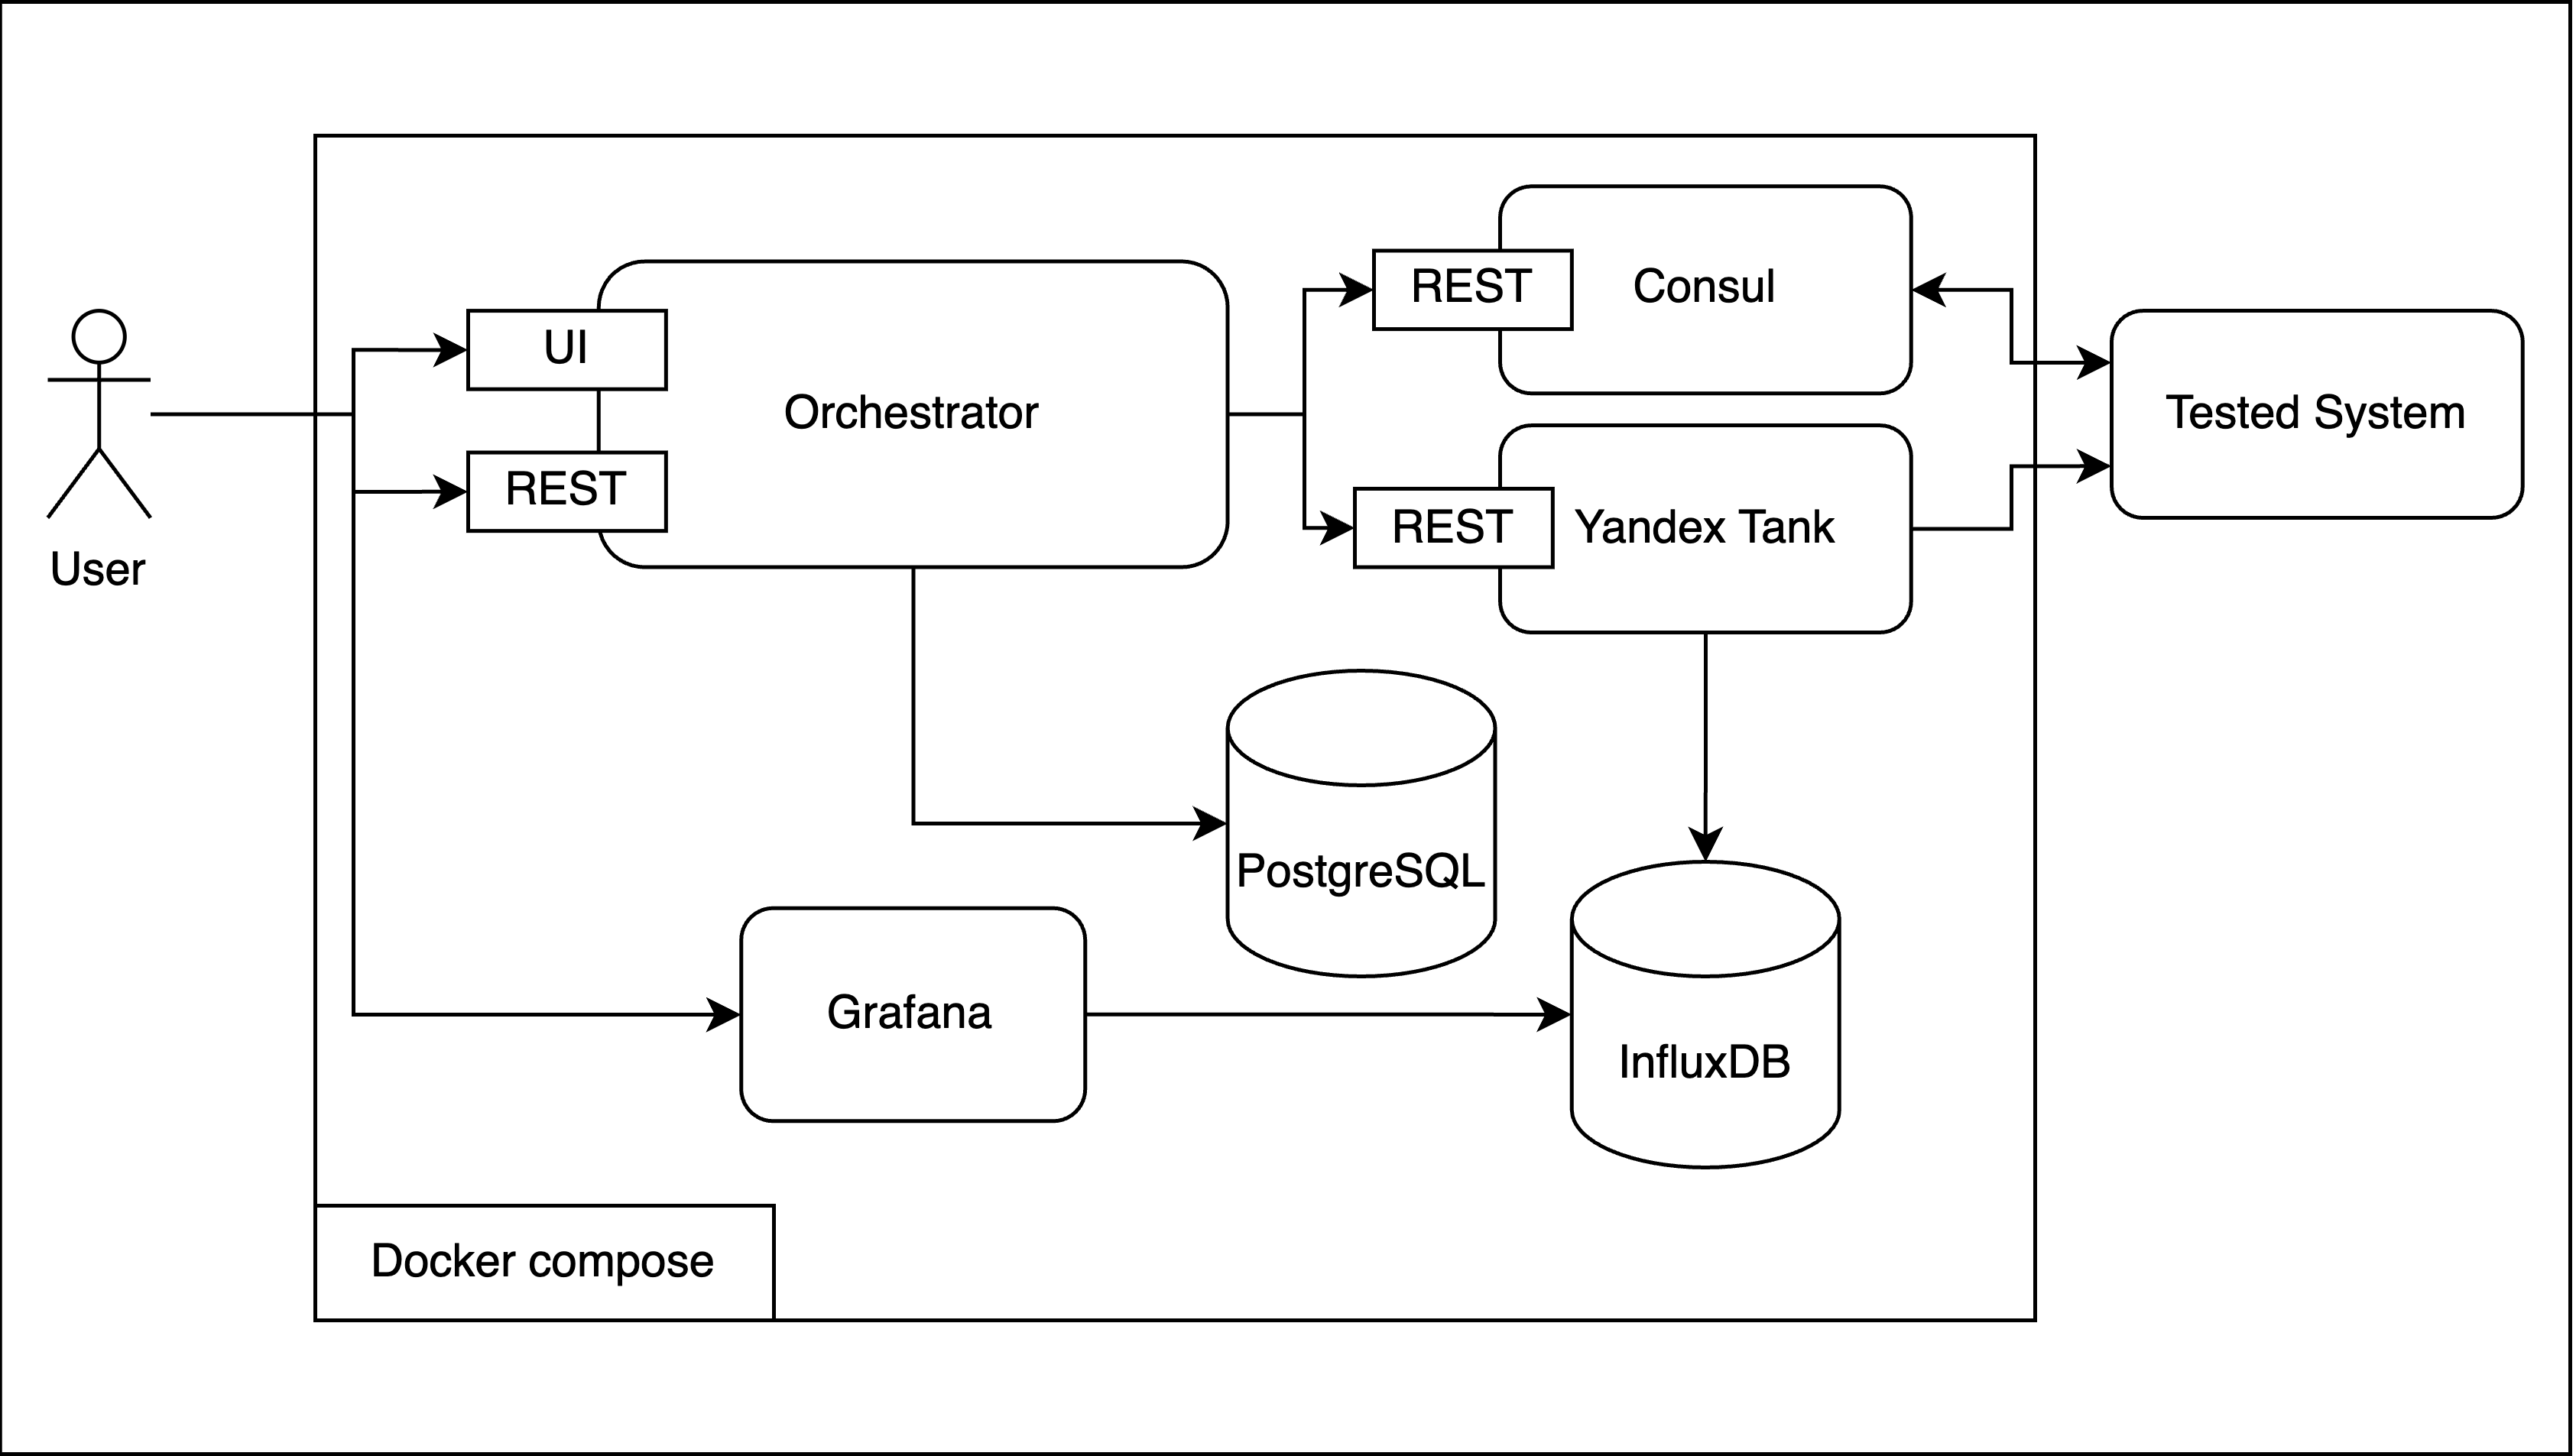
\includegraphics[height=\textheight,width=\textwidth,keepaspectratio]{architecture.png}
    \caption{Architecture of the system}
    \label{fig:architecture}
\end{figure}

\section{System Components}\label{sec:system-components}
This section discusses all the tools and technologies used in the systems, as well as the reasons why they are appropriate for the project.
\subsection{Yandex Tank API}\label{subsec:ya-api}
Yandex Tank is popular open source solution for load testing. It has convinient format of load testing configuration via YAML files. Also it can generate more the 100000 requests per seconds. But it does not provide ability to manipulate load test flow and can't be easily injected into automated web systems. Therefore, Yandex Tank API was used. It is wrapper aroung yandex tank and allows to start, stop, pause, resume load test. Additionally, it provides user-friendly REST API. All test results are saved into time series database InfluxDB described in subsection \ref{subsec:influx}

\subsection{InfluxDB}\label{subsec:influx}
The load test result is a timeline of application stats. InfluxDB is the tool that's optimized for storing that type of data. It does not require any external dependencies and it is written in Rust programming language, so it works fast. Additionaly, Yandex Tank support this database and can write results directly to it.

\subsection{PostgreSQL}\label{subsec:postgre}
For storage of load testing scenarios, history of exectutions and configuration of reliability patterns the PostgreSQL is used. This is a popular relative database management system (DBMS) that supports a wide range of data types, and the most significant for us is its support for JSON data type. In the implementation section, the entity-relationship model of the tables will be presented.

\subsection{Kafka}\label{subsec:kafka}
If a change of configuration of the reliability patterns occurs as an event, the system needs to be able to store a stream of these event. Additionally, it is needed to share this stream with the tested service, so that it can make changes to these parameters in its implementation of the pattern. A message broker system Kafka is well-suited for this purpose because it is optimized for storing stream of events.

\subsection{Grafana}\label{subsec:grafana}
Grafana is a tool used for visualizing test results. It can be integrated with InfluxDB and allows it to visualize time series data from that DBMS. Additionally, Grafana has a RESTful API that allows users to create and managed charts through HTTP requests.

\subsection{Orchestrator}\label{subsec:orchestrator}
For improved user experience, the Orchestrator User Interface (UI) is used as the primary user interface for the Orchestrator service \ref{subsec:orchestrator}. The UI provides forms for creating load test scenarios, executing load test and configuring reliability patterns. In addition, it visualises all stored scenarios, their executions and allows to change configuration of patterns.
\graphicspath{{figs/}} %path to images
\chapter{Implementation (draft)}
\label{ch:lr}
\chaptermark{Fourth Chapter Heading}

\definecolor{codegreen}{rgb}{0,0.6,0}
\definecolor{codegray}{rgb}{0.5,0.5,0.5}
\definecolor{codepurple}{rgb}{0.58,0,0.82}
\definecolor{backcolour}{rgb}{0.95,0.95,0.92}

\lstdefinestyle{mystyle}{
    backgroundcolor=\color{backcolour},
    commentstyle=\color{codegreen},
    keywordstyle=\color{magenta},
    numberstyle=\tiny\color{codegray},
    stringstyle=\color{codepurple},
    basicstyle=\ttfamily\footnotesize,
    breakatwhitespace=false,
    breaklines=true,
    captionpos=b,
    keepspaces=true,
    numbers=left,
    numbersep=5pt,
    showspaces=false,
    showstringspaces=false,
    showtabs=false,
    tabsize=2
}
\lstset{style=mystyle}


The following chapter provides implementation details for the system, including some issues that arose during development and the solutions to these issues.

\section{Component communication}\label{sec:communication}


\section{Entity-Relationship Diagram}

\begin{figure}[t]
    \centering
    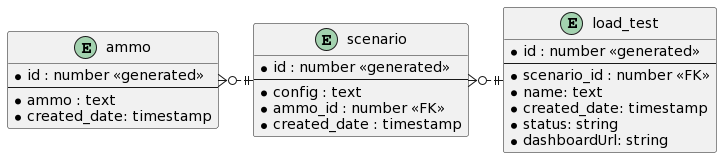
\includegraphics[height=\textheight,width=\textwidth,keepaspectratio]{erl.png}
    \caption{Entity-Relationship Diagram}
    \label{fig:erl}
\end{figure}


\section{Execute test scenario}

\begin{figure}[t]
    \centering
    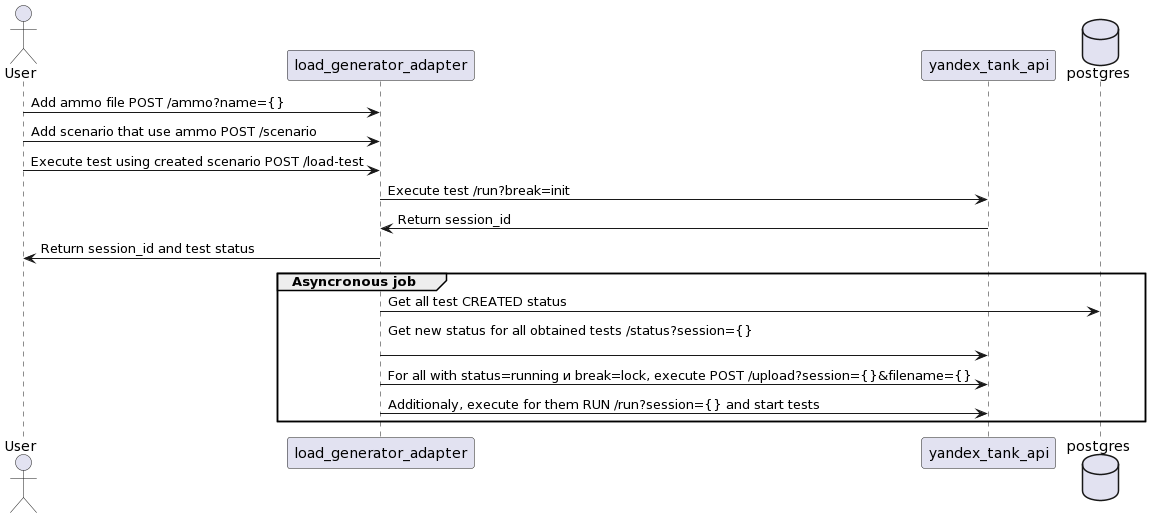
\includegraphics[height=\textheight,width=\textwidth,keepaspectratio]{diagram.png}
    \caption{Execute test scenario}
    \label{fig:test_scenario}
\end{figure}


\lstinputlisting[language=Octave]{code/docker-compose.yaml}
\usepackage{graphicx}


\chapter{Evaluation and Discussion}
\label{ch:eval}
\begin{longtable}{c|c}
    \caption[This is the title I want to appear in the List of Tables]{Simulation Parameters} \label{table:fifsimulation_params} \\
    \hline
    A                                     & B                               \\
    \hline
    \endfirsthead
    \multicolumn{2}{@{}l}{} \\
    \hline
    A                                     & B                               \\
    \hline
    \endhead
    \hline
    \textbf{Parameter}                    & \textbf{Value}                  \\
    \hline
    Number of vehicles                    & $|\mathcal{V}|$                 \\
    \hline
    Number of RSUs                        & $|\mathcal{U}|$                 \\
    \hline
    RSU coverage radius                   & 150 m                           \\
    \hline
    V2V communication radius              & 30 m                            \\
    \hline
    Smart vehicle antenna height          & 1.5 m                           \\
    \hline
    RSU antenna height                    & 25 m                            \\
    \hline
    Smart vehicle maximum speed           & $v_{\max}$ m/s                  \\
    \hline
    Smart vehicle minimum speed           & $v_{\min}$ m/s                  \\
    \hline
    Common smart vehicle cache capacities & $[50, 100, 150, 200, 250]$ mb   \\
    \hline
    Common RSU cache capacities           & $[5000,1000,1500,2000,2500]$ mb \\
    \hline
    Common backhaul rates                 & $[75, 100, 150]$ mb/s           \\
    \hline
\end{longtable}

\begin{figure}[hbt]
    \centering
    
\includegraphics[]{figs/inno.png}
    \caption{One kernel at $x_s$ (\emph{dotted kernel}) or two kernels at
        $x_i$ and $x_j$ (\textit{left and right}) lead to the same summed estimate
        at $x_s$. This shows a figure consisting of different types of
        lines. Elements of the figure described in the caption should be set in
        italics, in parentheses, as shown in this sample caption.}
    \label{fig:fifex}
\end{figure}

\ldots

\usepackage{graphicx}


\chapter{Conclusion}
\label{chap:conclusion}
\begin{longtable}{c|c}
    \caption[This is the title I want to appear in the List of Tables]{Simulation Parameters} \label{table:sixsimulation_params} \\
    \hline
    A                                     & B                               \\
    \hline
    \endfirsthead
    \multicolumn{2}{@{}l}{} \\
    \hline
    A                                     & B                               \\
    \hline
    \endhead
    \hline
    \textbf{Parameter}                    & \textbf{Value}                  \\
    \hline
    Number of vehicles                    & $|\mathcal{V}|$                 \\
    \hline
    Number of RSUs                        & $|\mathcal{U}|$                 \\
    \hline
    RSU coverage radius                   & 150 m                           \\
    \hline
    V2V communication radius              & 30 m                            \\
    \hline
    Smart vehicle antenna height          & 1.5 m                           \\
    \hline
    RSU antenna height                    & 25 m                            \\
    \hline
    Smart vehicle maximum speed           & $v_{\max}$ m/s                  \\
    \hline
    Smart vehicle minimum speed           & $v_{\min}$ m/s                  \\
    \hline
    Common smart vehicle cache capacities & $[50, 100, 150, 200, 250]$ mb   \\
    \hline
    Common RSU cache capacities           & $[5000,1000,1500,2000,2500]$ mb \\
    \hline
    Common backhaul rates                 & $[75, 100, 150]$ mb/s           \\
    \hline
\end{longtable}

\begin{figure}[hbt]
    \centering
    
\includegraphics[]{figs/inno.png}
    \caption{One kernel at $x_s$ (\emph{dotted kernel}) or two kernels at
        $x_i$ and $x_j$ (\textit{left and right}) lead to the same summed estimate
        at $x_s$. This shows a figure consisting of different types of
        lines. Elements of the figure described in the caption should be set in
        italics, in parentheses, as shown in this sample caption.}
    \label{fig:sixex}
\end{figure}

\ldots


%% REFERENCES
\printbibliography[heading=bibintoc,title={Bibliography cited}]

%\appendix
\chapter{Extra Stuff}
\blindtext

\chapter{Even More Extra Stuff}
\blindtext
\end{document}

